\documentclass[a4paper,10pt]{article}
\usepackage[left=2.5cm,right=2.5cm,top=2.5cm,bottom=2.5cm]{geometry}
\usepackage{amsmath}
\usepackage{amssymb}
\usepackage{parskip}
\usepackage{mathtools}
\usepackage{graphicx}
\usepackage[hidelinks]{hyperref}

\graphicspath{{../../images/}}


\begin{document}

% Title
\begingroup
\centering
\LARGE Multivariable Calculus Self-Learning Module\\[1em]
\large Exercises\par
\vspace{32pt}
\endgroup

\tableofcontents

\clearpage

\section{Exercise}

Calculate the length of curve $C$, where $C$ is the curve:
\[
    t \mapsto (\cos(t) + t\sin(t), \, \sin(t) - t\cos(t))
\]
for $0\leq t \leq 2\pi$.

\begin{figure}[!ht]
    \centering
    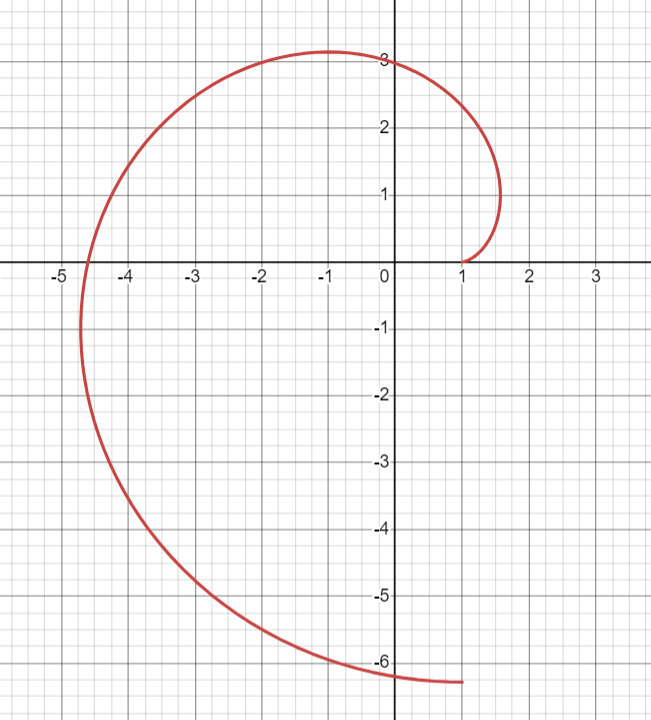
\includegraphics[scale=0.5]{ex_1.png}
\end{figure}

\subsection{Hint}
There is a formula for calculating the length of the curve. You must know this one! The formula is of the form:
\[
    \int_{\ldots}^{\ldots} |\ldots|\,dt
\]

\subsection{Hint}
The formula for the length is:
\[
    \int_{0}^{2\pi} |f'(t)|\,dt
\]

\subsection{Hint}
\begin{align*}
    f'(t) & = \frac{d}{dt} (\cos(t) + t\sin(t), \, \sin(t) - t\cos(t))         \\
          & = (-\sin(t) + \sin(t) + t\cos(t), \, \cos(t) - \cos(t) + t\sin(t)) \\
          & = (t\cos(t), \, t\sin(t))
\end{align*}
So
\begin{align*}
    |f'(t)| & = \sqrt{t^2\cos^2(t) + t^2\sin^2(t)} \\
            & = \sqrt{t^2}                         \\
            & = |t|
\end{align*}

\subsection{Solution}
Since $t \geq 0$, we have $|t| = t$, so:
\begin{align*}
    \int_{0}^{2\pi} |f'(t)|\,dt & = \int_{0}^{2\pi} t \, dt                \\
                                & = \left[ \frac{t^2}{2}\right]_{0}^{2\pi} \\
                                & = 2\pi^2
\end{align*}

\clearpage

\section{Exercise}

Consider the curve $C$ given by $f(x,y) = 0$, where
\[
    f(x,y) = (x-y)^2 + 4(x+y) - 4
\]
Determine the point on $C$ at which $x+y$ is maximal.

\subsection{Hint}
We want to maximize $g(x,y) = x+y$ subject to the constraint $f(x,y)=0$. Use Lagrange.

\subsection{Hint}
Solve the equation $\nabla g = \lambda\nabla f$.

\subsection{Solution}
\[
    \nabla g(x,y) = \begin{pmatrix} 1 \\ 1 \end{pmatrix}
\]
\[
    \nabla f(x,y) = \begin{pmatrix} 2(x-y) + 4 \\ -2(x-y) + 4 \end{pmatrix}
\]
So
\[
    \begin{pmatrix} 1 \\ 1 \end{pmatrix} = \lambda \begin{pmatrix} 2(x-y) + 4 \\ -2(x-y) + 4 \end{pmatrix}
\]
Note that $\lambda = 0$ gives
\[
    \begin{pmatrix} 1 \\ 1 \end{pmatrix} = \begin{pmatrix} 0 \\ 0 \end{pmatrix}
\]
which is a contradiction, so $\lambda \neq 0$ and we get the system:
\[
    \begin{cases}
        2(x-y) + 4 = \dfrac{1}{\lambda} \\ \\
        -2(x-y) + 4 = \dfrac{1}{\lambda}
    \end{cases}
\]
Subtracting the two equations gives:
\[
    2(x-y) + 4 + 2(x-y) - 4 =  \frac{1}{\lambda} - \frac{1}{\lambda} \iff 4(x-y) = 0 \iff x = y
\]
Since we are looking for the point that maximizes $x+y$ on $C$, we substitute $y=x$ in $f(x,y)=0$:
\[
    (x-x)^2 + 4(x+x) - 4 = 0 \iff 8x = 4 \iff x = \frac{1}{2}
\]
So
\[
    (x, y) = \left(\frac{1}{2}, \frac{1}{2}\right)
\]
and the maximum is
\[
    g\left(\frac{1}{2}, \frac{1}{2}\right) = 1.
\]

\clearpage

\section{Exercise}

Consider the function
\[
    f(x,y,z) = \frac{1}{x} + \frac{1}{8y} + \frac{1}{27z}.
\]
Find the point on the unit sphere (i.e. the sphere centered at $(0, 0, 0)$ of radius $1$) at which $f$ is maximal and the point at which it is minimal. Calculate also these maximum and minimum values.

\subsection{Hint}
The surface of a sphere centered at $(x_0, y_0, z_0)$ of radius $R$ has the formula
\[
    (x-x_0)^2 + (y-y_0)^2 + (z-z_0)^2 = R^2
\]

\subsection{Hint}
Let
\[
    g(x,y,z) = x^2 + y^2 + z^2 - 1.
\]
We want to maximize $f(x,y,z)$ given the constraint $g(x,y,z) = 0$. Use Lagrange.

\subsection{Hint}
Solve the equation $\nabla f = \lambda\nabla g$.

\subsection{Hint}
\[
    \nabla f(x,y,z) = \begin{pmatrix}
        -\dfrac{1}{x^2} \\ \\ -\dfrac{1}{8y^2} \\ \\ -\dfrac{1}{27z^2}
    \end{pmatrix}
\]

\[
    \nabla g(x,y,z) = \begin{pmatrix}
        2x \\ 2y \\ 2z
    \end{pmatrix}
\]
So
\[
    \begin{pmatrix}
        -\dfrac{1}{x^2} \\ \\ -\dfrac{1}{8y^2} \\ \\ -\dfrac{1}{27z^2}
    \end{pmatrix}
    = \lambda
    \begin{pmatrix}
        2x \\ 2y\\ 2z
    \end{pmatrix}
\]
Note that the left-hand side is always non-zero, so $\lambda \neq 0$. Hence:
\[
    \begin{cases}
        -\dfrac{1}{x^2} = 2\lambda x  \\ \\
        -\dfrac{1}{8y^2} = 2\lambda y \\ \\
        -\dfrac{1}{27z^2} = 2\lambda z
    \end{cases} \iff
    \begin{cases}
        x^3 = -\dfrac{1}{2\lambda}       \\ \\
        y^3 = -\dfrac{1}{8\cdot2\lambda} \\ \\
        z^3 = -\dfrac{1}{27\cdot 2\lambda}
    \end{cases} \iff
    \begin{cases}
        x = -\sqrt[3]{\dfrac{1}{2\lambda}}             \\ \\
        y = -\dfrac{1}{2}\sqrt[3]{\dfrac{1}{2\lambda}} \\ \\
        z = -\dfrac{1}{3}\sqrt[3]{\dfrac{1}{2\lambda}}
    \end{cases} \iff
    \begin{cases}
        x = -\sqrt[3]{\dfrac{1}{2\lambda}} \\ \\
        y = -\dfrac{1}{2} \cdot x          \\ \\
        z = -\dfrac{1}{3} \cdot x
    \end{cases}
\]

\subsection{Hint}
The points lie on the unit sphere, so $x^2+y^2+z^2=1$ must also hold.

\subsection{Solution}
\begin{align*}
    x^2 + \left(-\dfrac{1}{2}\cdot x\right)^2 + \left(-\dfrac{1}{3}\cdot x\right)^2 & = 1                \\
    \iff x^2\cdot\left(1 + \dfrac{1}{4} + \dfrac{1}{9}\right)                       & = 1                \\
    \iff x^2\cdot \dfrac{49}{36}                                                    & = 1                \\
    \iff x^2                                                                        & = \dfrac{36}{49}   \\
    \iff x                                                                          & = \pm \dfrac{6}{7}
\end{align*}
We get two solutions:
\begin{align*}
    x & = \dfrac{6}{7}                          \\
    y & = -\dfrac{1}{2} \cdot x = -\dfrac{3}{7} \\
    z & = -\dfrac{1}{3} \cdot x = -\dfrac{2}{7}
\end{align*}
and
\begin{align*}
    x & =  -\dfrac{6}{7}                       \\
    y & = -\dfrac{1}{2} \cdot x = \dfrac{3}{7} \\
    z & = -\dfrac{1}{3} \cdot x = \dfrac{2}{7}
\end{align*}
In order to determine which one gives the minimum and which one the maximum, we substitute in $f$:
\begin{align*}
    f\left(\dfrac{6}{7}, -\dfrac{3}{7}, -\dfrac{2}{7}\right) & = \frac{1}{-6/7} + \frac{1}{8\cdot(-3/7)} + \frac{1}{27\cdot (-2/7)} \\
                                                             & = -\frac{7}{6} - \frac{7}{24} - \frac{7}{54}                         \\
                                                             & = -\frac{373}{216}
\end{align*}
and
\begin{align*}
    f\left(-\dfrac{6}{7}, \dfrac{3}{7}, \dfrac{2}{7}\right) & = \frac{1}{6/7} + \frac{1}{8\cdot 3/7} + \frac{1}{27\cdot 2/7} \\
                                                            & = \frac{7}{6} + \frac{7}{24} + \frac{7}{54}                    \\
                                                            & = \frac{373}{216}
\end{align*}
So $f$ achieves a maximum value of $373/216$ at
\[
    \left(-\dfrac{6}{7}, \dfrac{3}{7}, \dfrac{2}{7}\right)
\]
and a minimum value of $-373/216$ at
\[
    \left(\dfrac{6}{7}, -\dfrac{3}{7}, -\dfrac{2}{7}\right).
\]

\clearpage

\section{Exercise}

Consider the function
\[
    f(x,y) = \frac{x^2 + y^2}{xy}
\]
defined on the set
\[
    K = \{(x,y): 0 < x \leq 1, 0 < y \leq 1\}.
\]
Determine where $f$ assumes its minimum, and what that minimum value is.

\subsection{Hint}
Calculate $\nabla f$.

\subsection{Hint}
\begin{align*}
    \frac{\partial f}{\partial x} & = \left(\frac{xy\cdot 2x - (x^2+y^2)\cdot y}{x^2y^2}\right) \\
                                  & = \frac{x^2y - y^3}{x^2y^2}                                 \\
                                  & = \frac{x^2 - y^2}{x^2y}
\end{align*}
By symmetry, we have:
\[
    \frac{\partial f}{\partial y} = \frac{y^2 - x^2}{xy^2}
\]
So
\[
    \nabla f(x,y) = \begin{pmatrix}
        \dfrac{\partial f}{\partial x} \\ \\ \dfrac{\partial f}{\partial y}
    \end{pmatrix} = \begin{pmatrix}
        \dfrac{x^2 - y^2}{x^2y} \\ \\ \dfrac{y^2 - x^2}{xy^2}
    \end{pmatrix}
\]

\subsection{Hint}
Solve $\nabla f = 0$.

\subsection{Hint}
\[
    \begin{pmatrix}
        \dfrac{x^2 - y^2}{x^2y} \\ \\ \dfrac{y^2 - x^2}{xy^2}
    \end{pmatrix} = 0 \iff x^2 - y^2 = 0 \iff x = \pm y
\]

\subsection{Solution}
Note that since $x, y > 0$ on $K$, we cannot have $x = -y$. Substituting $y=x$ in $f$ we get:
\[
    f(x,x) = \frac{x^2 + x^2}{x^2} = 2
\]
So $f$ achieves its minimum value 2 on the entire line segment $x=y$, $0 < x \leq 1, 0 < y \leq 1$.

\begin{figure}[!ht]
    \centering
    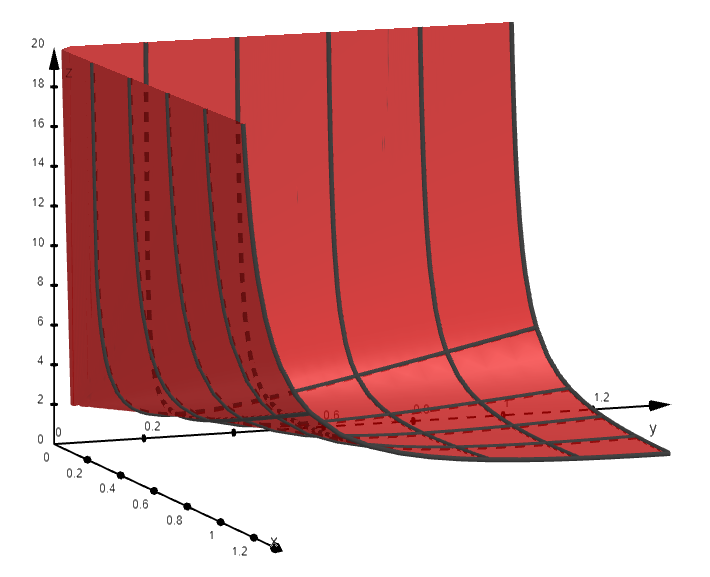
\includegraphics[scale=0.5]{ex_4.png}
\end{figure}

\clearpage

\section{Exercise}
Consider the surface $S$ defined by $f(x,y,z)=0$, where
\[
    f(x,y,z) = x^2 + y^2 + z^2 + 3xy - z - 11
\]
\begin{enumerate}
    \item Check that $A = (1,1,3)$ lies on $S$.
    \item Give an equation of the form $\alpha x+\beta y+\gamma z=\delta$ describing the tangent plane to $S$ at point $A$.
\end{enumerate}

\subsection{Hint}
1. Substitute $x=1$, $y=1$, $z=3$ in $f$ to get:
\[
    1^2 + 1^2 + 3^2 + 3\cdot 1\cdot 1 - 3 - 11 = 0.
\]

\subsection{Hint}
2. There are several ways to go about this, but in most (if not all) you need to compute $\nabla f$ at the point $A$.

\subsection{Hint}
\[
    \nabla f(x,y,z) = \begin{pmatrix}
        \dfrac{\partial f}{\partial x} \\ \\ \dfrac{\partial f}{\partial y} \\ \\ \dfrac{\partial f}{\partial z}
    \end{pmatrix} = \begin{pmatrix}
        2x+3y \\ 3x+2y \\ 2z-1
    \end{pmatrix}
\]
So
\[
    \nabla f(1,1,3) = \begin{pmatrix}
        2\cdot 1+3\cdot 1 \\ 3\cdot 1+2\cdot 1 \\ 2\cdot 3-1
    \end{pmatrix} = \begin{pmatrix}
        5 \\ 5 \\ 5
    \end{pmatrix}
\]

\subsection{Hint}
The gradient of $f$ at $A$ is a vector orthogonal to the tangent plane to $S$ at point $A$. How do you find an equation of a plane if you know a vector orthogonal to it and a point on it?

\subsection{Solution}
The tangent plane is perpendicular to the vector $\nabla f(1, 1, 3) = (5, 5, 5)$ and passes through the point $(1, 1, 3)$, so its equation is:
\[
    5\cdot(x-1) + 5\cdot (y-1) + 5 \cdot (z-3) = 0 \iff 5x+5y+5z = 25
\]

\emph{\textbf{Remark:} There is also a formula given in the book as the linearization of $f$ at $A = (x_0, y_0, z_0)$:}
\[
    L(x,y,z) = f(A) + f_x(A)\cdot (x - x_0) + f_y(A)\cdot (y - y_0) + f_z(A)\cdot (z - z_0)
\]
\emph{(this is essentially a first order Taylor expansion). The formula will yield the exact same answer. However, applying formulas without understanding is like eating your food without chewing!}

\clearpage

\section{Exercise}

Consider the plane $P$ which contains the points $A = (1, 1, 1)$, $B = (2, 3, 9)$, $C = (3, 5, 4)$. Try to think of as many was as possible to determine the equation $\alpha x + \beta y + \gamma z = \delta$ of this plane.

\subsection{Method 1}
Just substitute the coordinates of the 3 points in $\alpha x + \beta y + \gamma z = \delta$ and solve for $\alpha$, $\beta$, $\gamma$, $\delta$.

\subsection{Solution 1}
\begin{align*}
     & \begin{cases}
           \alpha + \beta + \gamma = \delta                                        \\
           2\alpha + 3\beta + 9\gamma = \delta & |\quad R_2 \leftarrow R_2 - 2 R_1 \\
           3\alpha + 5\beta + 4\gamma = \delta & |\quad R_3 \leftarrow R_3 - 3 R_1
       \end{cases} \\ \iff &
    \begin{cases}
        \alpha + \beta + \gamma = \delta                                        \\
        \beta + 7\gamma = -\delta                                               \\
        2\beta + \gamma = -2\delta & |\quad R_3 \leftarrow R_2 - \frac{1}{2}R_3
    \end{cases}    \\ \iff &
    \begin{cases}
        \alpha + \beta + \gamma = \delta \\
        \beta + 7\gamma = -\delta        \\
        \frac{13}{2}\gamma = 0
    \end{cases}                                           \\ \iff &
    \begin{cases}
        \alpha = 2\delta \\
        \beta = -\delta  \\
        \gamma = 0
    \end{cases}
\end{align*}

Note that $\delta$ is a free variable here, and
\[
    2\delta \cdot x -\delta \cdot y + 0\cdot z = \delta
\]
defines the same plane for any $\delta \neq 0$ (for $\delta=0$ we just get $0=0$ which is satisfied by any $x,y,z$, i.e. we don't get a plane but the entire $\mathbb{R}^3$). So we can choose for example $\delta =1$ to get the following equation for $P$:
\[
    2x - y = 1
\]

\begin{figure}[!ht]
    \centering
    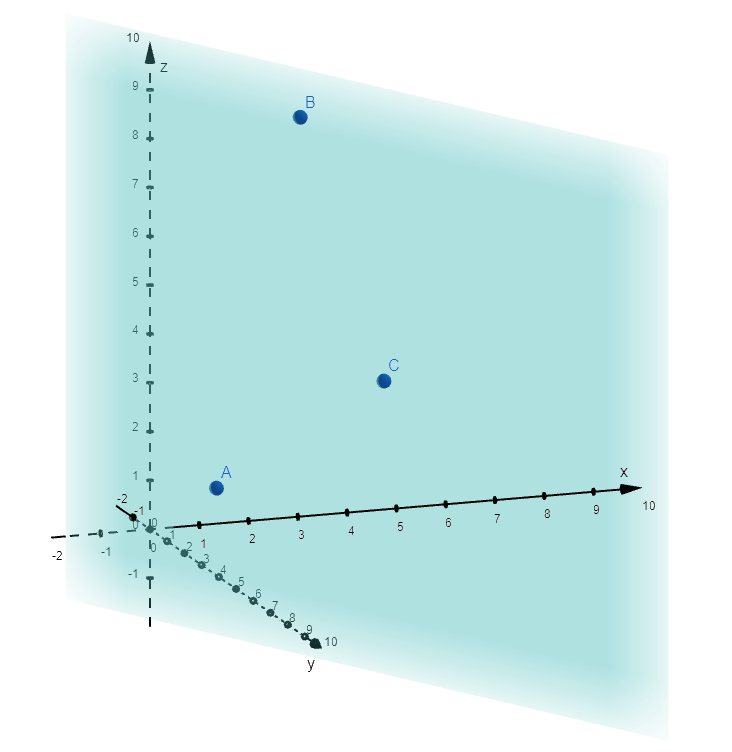
\includegraphics[scale=0.5]{ex_6.png}
\end{figure}

\subsection{Method 2}
Make the vectors $\overrightarrow{AB}$, $\overrightarrow{AC}$ and compute the vector $\overrightarrow{AB} \times \overrightarrow{AC}$. Then...

\subsection{Solution 2}
\[
    \overrightarrow{AB} = \overrightarrow{B} - \overrightarrow{A} = (2, 3, 9) - (1, 1, 1) = (1, 2, 8)
\]
\[
    \overrightarrow{AC} = \overrightarrow{C} - \overrightarrow{A} = (3, 5, 4) - (1, 1, 1) = (2, 4, 3)
\]
\begin{align*}
    \overrightarrow{AB} \times \overrightarrow{AC} & = \begin{vmatrix}
                                                           1 & 2 & 8 \\ 2 & 4 & 3 \\ e_x & e_y & e_z
                                                       \end{vmatrix} \\ & =  \begin{vmatrix}
        2 & 8 \\ 4 & 3
    \end{vmatrix} \cdot e_x - \begin{vmatrix}
        1 & 8 \\ 2 & 3
    \end{vmatrix} \cdot e_y + \begin{vmatrix}
        1 & 2 \\ 2 & 4
    \end{vmatrix} \cdot e_z \\
                                                   & = -26 \cdot e_x + 13\cdot e_y + 0\cdot e_z \\
                                                   & = (-26, 13, 0)
\end{align*}
Now $\overrightarrow{AB} \times \overrightarrow{AC}$ is normal to $P$ and $A$ lies on $P$, so we get the following equation for $P$:
\[
    -26\cdot(x -1) + 13\cdot (y-1) + 0\cdot (z-1) = 0 \iff -26x + 13y = -13
\]

\subsection{Method 3}
Find a vector $(\alpha, \beta, \gamma)$ that is orthogonal to $\overrightarrow{AB}$, $\overrightarrow{AC}$ by solving the system
\begin{align*}
    \overrightarrow{AB}\cdot (\alpha, \beta, \gamma) & = 0 \\
    \overrightarrow{AC}\cdot (\alpha, \beta, \gamma) & = 0
\end{align*}
Then...

\subsection{Solution 3}
\begin{align*}
         & \begin{cases}
               (1, 2, 8) \cdot (\alpha, \beta, \gamma) = 0 \\
               (2, 4, 3) \cdot (\alpha, \beta, \gamma) = 0
           \end{cases}                         \\
    \iff & \begin{cases}
               \alpha + 2\beta +8\gamma = 0                                        \\
               2\alpha + 4\beta + 3\gamma = 0 & | \quad R_2 \leftarrow R_2 - 2 R_1
           \end{cases} \\
    \iff & \begin{cases}
               \alpha + 2\beta +8\gamma = 0 \\
               -13\gamma = 0
           \end{cases}
    \\ \iff & \begin{cases}
        \alpha = -2\beta \\
        \gamma = 0
    \end{cases}
\end{align*}
Choose $\beta = 1$, so $(\alpha, \beta, \gamma) = (-2, 1, 0)$, and the equation for $P$ becomes:
\[
    -2\cdot x + 1\cdot y + 0\cdot z = \delta
\]
Substitute $(1, 1, 1)$ in the equation to find $\delta$:
\[
    \delta = -2 + 1 = -1
\]
So the equation for $P$ is:
\[
    -2x+y=-1
\]

\clearpage

\section{Exercise}

Find all points that are equidistant to the 3 points $A = (2, 2, 0)$, $B = (0, 3, 3)$, $C = (4, 0, 4)$.

\subsection{Hint}
Let $P=(x,y,z)$ be such a point. Write down equations for the distances of $P$ from $A,B,C$ to be equal, i.e.:
\[
    \left|\overrightarrow{PA}\right|^2 = \left|\overrightarrow{PB}\right|^2 = \left|\overrightarrow{PC}\right|^2
\]

\subsection{Hint}
\[
    \left|\overrightarrow{PA}\right|^2 = (x-2)^2 + (y-2)^2 +(z-0)^2,
\]
etc.

\subsection{Hint}
\begin{align*}
         & \ (x-2)^2 + (y-2)^2 + (z-0)^2    \\
    =    & \ (x-0)^2 + (y-3)^2 + (z-3)^2    \\
    =    & \ (x-4)^2 + (y-0)^2 + (z-4)^2    \\
    \iff &                                  \\
         & \ x^2 + y^2 + z^2 - 4x - 4y + 8  \\
    =    & \ x^2 + y^2 + z^2 - 6y - 6z + 18 \\
    =    & \ x^2 + y^2 + z^2 - 8x - 8z + 32 \\
    \iff &                                  \\
         & \ - 4x - 4y                      \\
    =    & \ - 6y - 6z + 10                 \\
    =    & \ - 8x - 8z + 24                 \\
    \iff &                                  \\
         & \ 2x + 2y                        \\
    =    & \ 3y + 3z - 10                   \\
    =    & \ 4x + 4z - 12                   \\
\end{align*}

\subsection{Hint}
Note that in fact we have 2 equations:
\[
    \begin{cases}
        2x + 2y = 3y + 3z - 10 \\
        2x + 2y = 4x + 4z - 12
    \end{cases} \iff \begin{cases}
        2x - y - 3z = -10 \\
        -2x + 2y - 4z = -12
    \end{cases}
\]
So the solution is the intersection of 2 planes, i.e. a line! How can we find the equation of the line in parametric form?

\subsection{Hint}
This is now a linear algebra problem.
\begin{align*}
     & \left(
    \begin{array}{c c c|c}
            2  & -1 & -3 & -10 \\
            -2 & 2  & -4 & -12 \\
        \end{array}
    \right) \quad | \quad R_2 \leftarrow R_2 + R_1       \\ \rightarrow
     & \left(
    \begin{array}{c c c|c}
            2 & -1 & -3 & -10 \\
            0 & 1  & -7 & -22 \\
        \end{array}
    \right) \quad | \quad R_1 \leftarrow R_1 + R_2       \\ \rightarrow
     & \left(
    \begin{array}{c c c|c}
            2 & 0 & -10 & -32 \\
            0 & 1 & -7  & -22 \\
        \end{array}
    \right) \quad | \quad R_1 \leftarrow \frac{1}{2} R_1 \\ \rightarrow
     & \left(
    \begin{array}{c c c|c}
            1 & 0 & -5 & -16 \\
            0 & 1 & -7 & -22 \\
        \end{array}
    \right)
\end{align*}
So
\[
    \begin{cases}
        x - 5z = -16 \\
        y - 7z = -22
    \end{cases} \iff \begin{cases}
        x = 5z - 16 \\
        y = 7z - 22
    \end{cases},
\]
where $z$ is free. So there is a line of points equidistant from $A, B, C$ given by the equation:
\[
    (x, y, z) = (5\lambda - 16, 7\lambda - 22, \lambda)
\]
for $\lambda\in\mathbb{R}$.

\clearpage

\section{Exercise}

Consider the following 5 points:
\[
    A = (0, 0, 0), \quad B = (2, 0, 0), \quad C = (4, 4, 0), \quad D = (4, 0, 4), \quad E = (0, 0, 4)
\]
Find all the points that are equidistant from $A,B,C,D,E$.

\subsection{Hint}
Let $P=(x,y,z)$ be such a point. Write down equations for the distances of $P$ from $A,B,C$ to be equal, i.e.:
\[
    \left|\overrightarrow{PA}\right|^2 = \left|\overrightarrow{PB}\right|^2 = \left|\overrightarrow{PC}\right|^2 = \left|\overrightarrow{PD}\right|^2 = \left|\overrightarrow{PE}\right|^2
\]

\subsection{Hint}
\[
    \left|\overrightarrow{PB}\right|^2 = (x-2)^2 + (y-0)^2 +(z-0)^2,
\]
etc.

\subsection{Hint}
\begin{align*}
         & \ (x-0)^2 + (y-0)^2 + (z-0)^2    \\
    =    & \ (x-2)^2 + (y-0)^2 + (z-0)^2    \\
    =    & \ (x-4)^2 + (y-4)^2 + (z-0)^2    \\
    =    & \ (x-4)^2 + (y-0)^2 + (z-4)^2    \\
    =    & \ (x-0)^2 + (y-0)^2 + (z-4)^2    \\
    \iff &                                  \\
         & \ x^2 + y^2 + z^2                \\
    =    & \ x^2 + y^2 + z^2 - 4x + 4       \\
    =    & \ x^2 + y^2 + z^2 - 8x - 8y + 32 \\
    =    & \ x^2 + y^2 + z^2 - 8x - 8z + 32 \\
    =    & \ x^2 + y^2 + z^2 - 8z + 16      \\
    \iff &                                  \\
         & \ 0                              \\
    =    & \ - 4x + 4                       \\
    =    & \ - 8x - 8y + 32                 \\
    =    & \ - 8x - 8z + 32                 \\
    =    & \ - 8z + 16                      \\
\end{align*}

\subsection{Solution}
We have:
\[
    0 = -4x + 4 \iff x=1
\]
For $x=1$:
\[
    0 = - 8x - 8y + 32 = -8y + 24 \iff y = 3
\]
For $x=1, y=3$:
\[
   0 =  - 8x - 8z + 32 \iff z = 3
\]
But now for $x=1$, $y=3$, $z=3$:
\[
    -8z + 16 = 0 \implies -8 = 0,
\]
contradiction! So there are no points equidistant from $A, B, C, D, E$.


\end{document}